Beim Reinforcement Learning setzt man intelligente Programme, welche auch Agenten genannt werden, ein. Hierbei gibt es keine Trainings-Daten. \cite{Nandy2018} Ein Agent trainiert um sich seiner Umgebung anzupassen und seine Leistung zu verbessern. \cite{Sarkar2018} \newline
	Er kennt den Zustand, in dem sich seine Umgebung befindet und führt Aktionen aus, um diesen zu verändern. Das Ausführen von Aktionen von einem Start- bis zu einem Endzustand nennt man Episode oder Prozess. \cite{Alpaydin2004}\newline  
	Die Umgebung kann eine 2D oder 3D Simulation eines Szenarios aus der echten Welt oder aus einem Spiel sein.  
	Die Wahl der Aktionen erfolgt durch Ausprobieren, da es sehr schwer ist von Beginn an vorauszusagen, welche Aktion in welchem Zustand ausgeführt werden muss. \cite{Nandy2018} Der Agent besitzt bereits zu Beginn bestimmte Strategien und Richtlinien, welche verbessert und angepasst werden. \cite{Sarkar2018}
	Abhängig von der Interaktion mit der Umgebung erhält der Agent von der Umgebung Belohnungen und Bestrafungen, meist in Form von plus und minus Punkten. \cite{Nandy2018} Diese führen zu einem Update der Strategien, um später mehr Belohnungen zu erhalten. \cite{Sarkar2018}\newline
	\begin{figure}[H]
		\centering
		
\includegraphics[width=5cm]{Bilder/Reinforcement.pdf}
		\caption{Umgebung mit Agent}
		\label{fig:abb6}
	\end{figure}
	Reinforcement Learning wird auch Lernen mit einem Kritiker genannt, da dem Modell im Lernprozess nicht vorgegeben wird was es tun soll. Erst nach dem Ausführen der Aktionen, wird eine Rückmeldung über diese an das Modell weitergegeben. \cite{Alpaydin2004}
	
	\subsection{Umgebung}
	Die Umgebung des Agenten kann mit bestimmten Eigenschaften beschrieben werden, diese werden im Folgenden erläutert. \cite{Nandy2018} \newline
	Ist die Umgebung deterministisch gibt es für jede Aktion nur einen Übergang zu einem anderen Zustand. Ist sie nicht-deterministisch sind mehrere Übergänge für jede Aktion möglich. \cite{Nandy2018}\newline
	Ist die Umgebung beobachtbar, können wie bei einem Schachspiel, alle Informationen über die Umgebung wahrgenommen werden. Wenn die Umgebung nur teilweise beobachtbar ist, sind bestimmte Informationen versteckt, wie zum Besipiel beim Poker die Handkarten der anderen Mitspieler. \cite{Nandy2018}\newline
	Eine Umgebung ist fortlaufend, wenn es mehr als eine Aktion gibt, um zum nächsten Zustand zu gelangen. Ist sie beschränkt, gibt es nur eine Aktion, die zum nächsten Zustand führt. \cite{Nandy2018}
	\begin{figure}[h!]
		\centering
		\includegraphics[width=8cm]{Bilder/Umgebung.pdf}
		\caption{beschränkte und fortlaufende Umgebung}
		\label{fig:abb7}
	\end{figure} \newline
	Es gibt multi-agent Umgebungen, die für Problemstellungen mit mehrere Umgebungen, verschiedenen Aufgaben und ähnlichen Entscheidungen geeignet sind. Hier gibt es oft mehr als eine Aktion, um zum nächsten Status zu gelangen. Dies wird durch Kommunikation zwischen den Agenten ermöglicht. Die Umgebung kann bei einer multi-agent Problemstellung dynamisch sein, was bedeutet, dass es Veränderungen der Umgebung an Interaktionsstellen geben kann. In single-agent Umgebungen gibt es nur eine Umgebung, da keine Kommunikation zwischen Agenten möglich ist. \cite{Nandy2018}
	\begin{figure}[H]
		\centering
		
\includegraphics[width=5cm]{Bilder/multiagent.pdf}
		\caption{Umgebung mit zwei Agenten}
		\label{fig:abb8}
	\end{figure}

	\subsection{Einsatzbereiche}	
	Reinforcement Learning wird in der Produktion von Robotern genutzt, um Objekte von einer Box in eine andere zu befördern. In der Lagerverwaltung werden Transportzeiten zwischen Lagern verringert und die Platznutzung im Lager durch Reinforcement Learning optimiert. Die Fahrzeugnutzung in der Lieferverwaltung kann damit ebenfalls optimiert werden. Im Finanzbereich wird unter Verwendung von Handelsstrategien die Buchhaltung unterstützt. \cite{Nandy2018}
	